\subsection{Aufgabe 1}

Wir sollten die Apparatur aufbauen und justieren. Dabei geht der Strahlengang  des Lichts von der Dampflampe aus durch die Kondensorlinse, in welcher das Licht gesammelt wird. Durch den darauf folgenden Spalt konnte man die Intensität des Lichts regulieren. Die Kollimatorlinse sollte ein möglichst parallelen Strahlengang erzeugen, welcher anschließend zum Prisma gelangt und dort gebrochen wird.
\\
\begin{center}
\begin{minipage}{\linewidth}
\centering
\makebox[0cm]{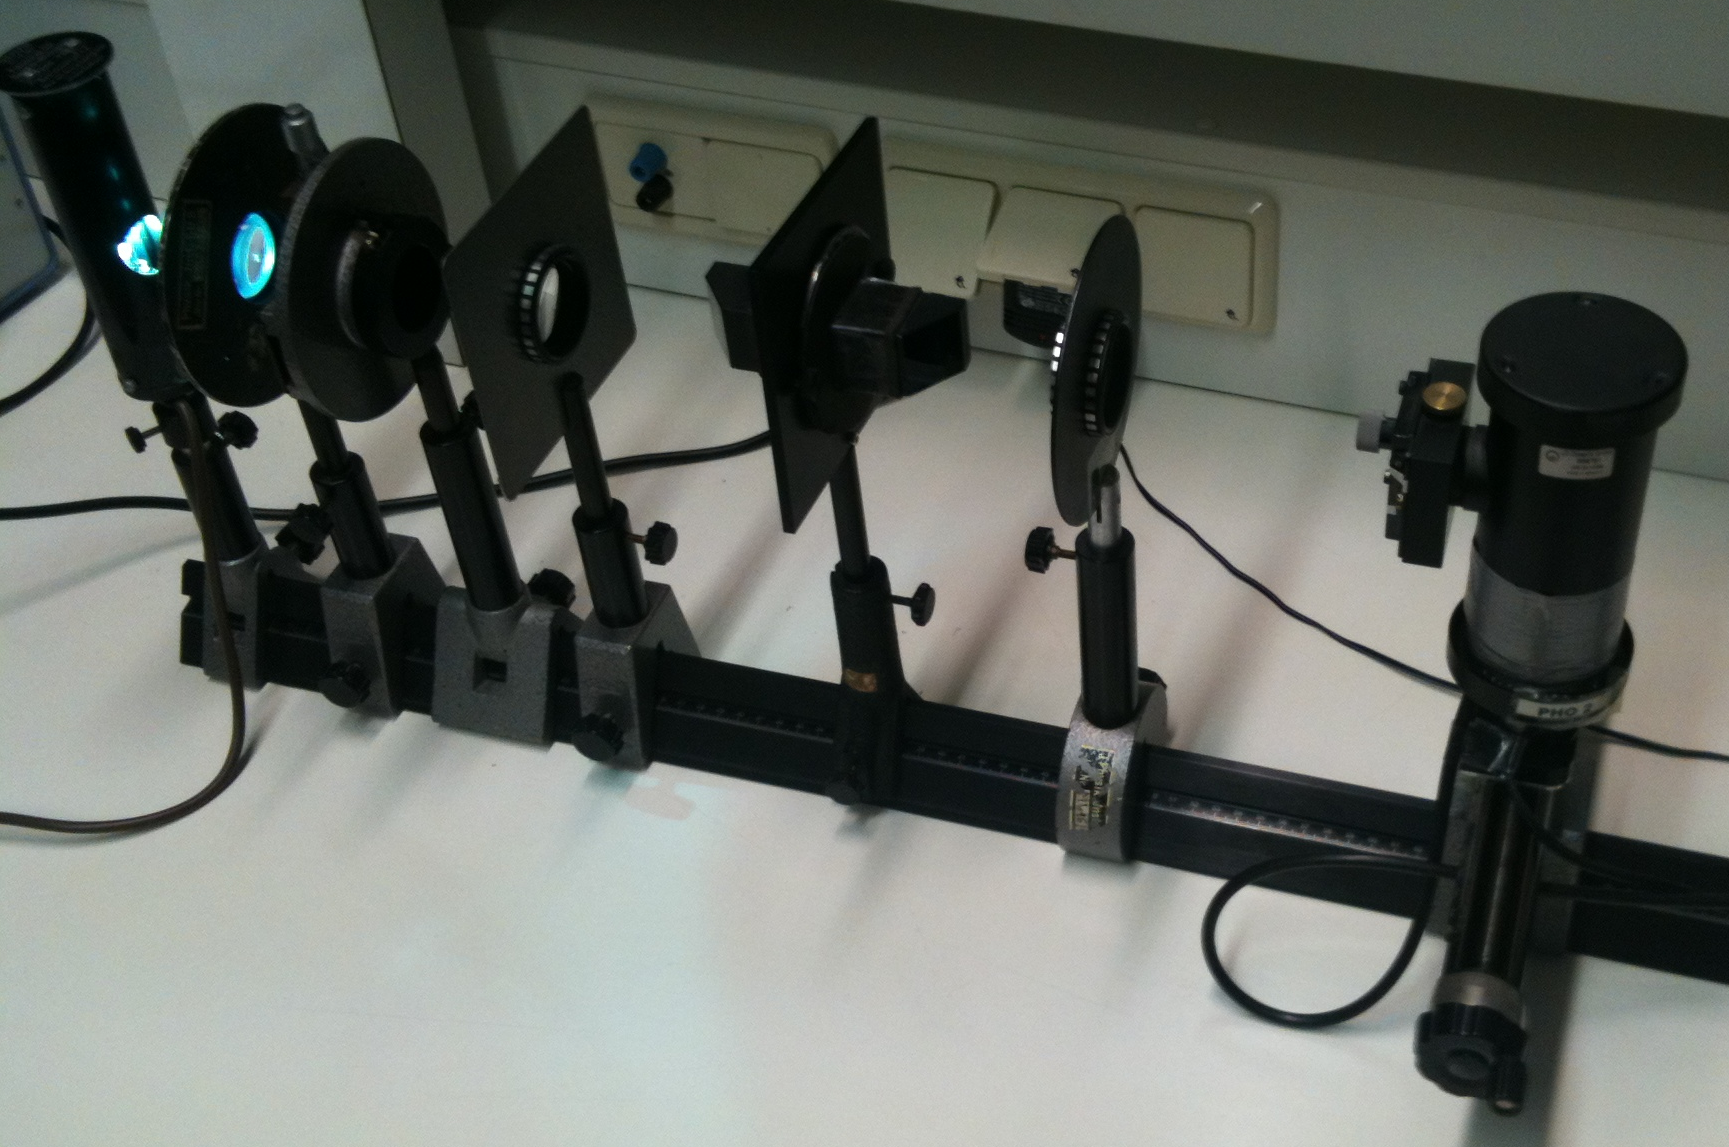
\includegraphics[width=\textwidth]{bilder/pho4}}
\captionof{figure}{Aufbau der Messapparatur (von Links: Hg-Dampflampe, Kondensorlinse, variabler Spalt, Kollimatorlinse, Dispersionsprisma, Achromator, (Kalium-)Photozelle}%
\label{ringe}
\end{minipage}
\end{center}